% Options for packages loaded elsewhere
\PassOptionsToPackage{unicode}{hyperref}
\PassOptionsToPackage{hyphens}{url}
%
\documentclass[
]{book}
\usepackage{amsmath,amssymb}
\usepackage{lmodern}
\usepackage{ifxetex,ifluatex}
\ifnum 0\ifxetex 1\fi\ifluatex 1\fi=0 % if pdftex
  \usepackage[T1]{fontenc}
  \usepackage[utf8]{inputenc}
  \usepackage{textcomp} % provide euro and other symbols
\else % if luatex or xetex
  \usepackage{unicode-math}
  \defaultfontfeatures{Scale=MatchLowercase}
  \defaultfontfeatures[\rmfamily]{Ligatures=TeX,Scale=1}
\fi
% Use upquote if available, for straight quotes in verbatim environments
\IfFileExists{upquote.sty}{\usepackage{upquote}}{}
\IfFileExists{microtype.sty}{% use microtype if available
  \usepackage[]{microtype}
  \UseMicrotypeSet[protrusion]{basicmath} % disable protrusion for tt fonts
}{}
\makeatletter
\@ifundefined{KOMAClassName}{% if non-KOMA class
  \IfFileExists{parskip.sty}{%
    \usepackage{parskip}
  }{% else
    \setlength{\parindent}{0pt}
    \setlength{\parskip}{6pt plus 2pt minus 1pt}}
}{% if KOMA class
  \KOMAoptions{parskip=half}}
\makeatother
\usepackage{xcolor}
\IfFileExists{xurl.sty}{\usepackage{xurl}}{} % add URL line breaks if available
\IfFileExists{bookmark.sty}{\usepackage{bookmark}}{\usepackage{hyperref}}
\hypersetup{
  pdftitle={Data gathering for Water Security: a contextualised approach},
  pdfauthor={Giacomo Butte},
  hidelinks,
  pdfcreator={LaTeX via pandoc}}
\urlstyle{same} % disable monospaced font for URLs
\usepackage{color}
\usepackage{fancyvrb}
\newcommand{\VerbBar}{|}
\newcommand{\VERB}{\Verb[commandchars=\\\{\}]}
\DefineVerbatimEnvironment{Highlighting}{Verbatim}{commandchars=\\\{\}}
% Add ',fontsize=\small' for more characters per line
\usepackage{framed}
\definecolor{shadecolor}{RGB}{248,248,248}
\newenvironment{Shaded}{\begin{snugshade}}{\end{snugshade}}
\newcommand{\AlertTok}[1]{\textcolor[rgb]{0.94,0.16,0.16}{#1}}
\newcommand{\AnnotationTok}[1]{\textcolor[rgb]{0.56,0.35,0.01}{\textbf{\textit{#1}}}}
\newcommand{\AttributeTok}[1]{\textcolor[rgb]{0.77,0.63,0.00}{#1}}
\newcommand{\BaseNTok}[1]{\textcolor[rgb]{0.00,0.00,0.81}{#1}}
\newcommand{\BuiltInTok}[1]{#1}
\newcommand{\CharTok}[1]{\textcolor[rgb]{0.31,0.60,0.02}{#1}}
\newcommand{\CommentTok}[1]{\textcolor[rgb]{0.56,0.35,0.01}{\textit{#1}}}
\newcommand{\CommentVarTok}[1]{\textcolor[rgb]{0.56,0.35,0.01}{\textbf{\textit{#1}}}}
\newcommand{\ConstantTok}[1]{\textcolor[rgb]{0.00,0.00,0.00}{#1}}
\newcommand{\ControlFlowTok}[1]{\textcolor[rgb]{0.13,0.29,0.53}{\textbf{#1}}}
\newcommand{\DataTypeTok}[1]{\textcolor[rgb]{0.13,0.29,0.53}{#1}}
\newcommand{\DecValTok}[1]{\textcolor[rgb]{0.00,0.00,0.81}{#1}}
\newcommand{\DocumentationTok}[1]{\textcolor[rgb]{0.56,0.35,0.01}{\textbf{\textit{#1}}}}
\newcommand{\ErrorTok}[1]{\textcolor[rgb]{0.64,0.00,0.00}{\textbf{#1}}}
\newcommand{\ExtensionTok}[1]{#1}
\newcommand{\FloatTok}[1]{\textcolor[rgb]{0.00,0.00,0.81}{#1}}
\newcommand{\FunctionTok}[1]{\textcolor[rgb]{0.00,0.00,0.00}{#1}}
\newcommand{\ImportTok}[1]{#1}
\newcommand{\InformationTok}[1]{\textcolor[rgb]{0.56,0.35,0.01}{\textbf{\textit{#1}}}}
\newcommand{\KeywordTok}[1]{\textcolor[rgb]{0.13,0.29,0.53}{\textbf{#1}}}
\newcommand{\NormalTok}[1]{#1}
\newcommand{\OperatorTok}[1]{\textcolor[rgb]{0.81,0.36,0.00}{\textbf{#1}}}
\newcommand{\OtherTok}[1]{\textcolor[rgb]{0.56,0.35,0.01}{#1}}
\newcommand{\PreprocessorTok}[1]{\textcolor[rgb]{0.56,0.35,0.01}{\textit{#1}}}
\newcommand{\RegionMarkerTok}[1]{#1}
\newcommand{\SpecialCharTok}[1]{\textcolor[rgb]{0.00,0.00,0.00}{#1}}
\newcommand{\SpecialStringTok}[1]{\textcolor[rgb]{0.31,0.60,0.02}{#1}}
\newcommand{\StringTok}[1]{\textcolor[rgb]{0.31,0.60,0.02}{#1}}
\newcommand{\VariableTok}[1]{\textcolor[rgb]{0.00,0.00,0.00}{#1}}
\newcommand{\VerbatimStringTok}[1]{\textcolor[rgb]{0.31,0.60,0.02}{#1}}
\newcommand{\WarningTok}[1]{\textcolor[rgb]{0.56,0.35,0.01}{\textbf{\textit{#1}}}}
\usepackage{longtable,booktabs,array}
\usepackage{calc} % for calculating minipage widths
% Correct order of tables after \paragraph or \subparagraph
\usepackage{etoolbox}
\makeatletter
\patchcmd\longtable{\par}{\if@noskipsec\mbox{}\fi\par}{}{}
\makeatother
% Allow footnotes in longtable head/foot
\IfFileExists{footnotehyper.sty}{\usepackage{footnotehyper}}{\usepackage{footnote}}
\makesavenoteenv{longtable}
\usepackage{graphicx}
\makeatletter
\def\maxwidth{\ifdim\Gin@nat@width>\linewidth\linewidth\else\Gin@nat@width\fi}
\def\maxheight{\ifdim\Gin@nat@height>\textheight\textheight\else\Gin@nat@height\fi}
\makeatother
% Scale images if necessary, so that they will not overflow the page
% margins by default, and it is still possible to overwrite the defaults
% using explicit options in \includegraphics[width, height, ...]{}
\setkeys{Gin}{width=\maxwidth,height=\maxheight,keepaspectratio}
% Set default figure placement to htbp
\makeatletter
\def\fps@figure{htbp}
\makeatother
\setlength{\emergencystretch}{3em} % prevent overfull lines
\providecommand{\tightlist}{%
  \setlength{\itemsep}{0pt}\setlength{\parskip}{0pt}}
\setcounter{secnumdepth}{5}
\usepackage{booktabs}
\usepackage{amsthm}
\makeatletter
\def\thm@space@setup{%
  \thm@preskip=8pt plus 2pt minus 4pt
  \thm@postskip=\thm@preskip
}
\makeatother
\ifluatex
  \usepackage{selnolig}  % disable illegal ligatures
\fi
\usepackage[]{natbib}
\bibliographystyle{apalike}

\title{Data gathering for Water Security: a contextualised approach}
\author{Giacomo Butte}
\date{2021-01-25}

\begin{document}
\maketitle

{
\setcounter{tocdepth}{1}
\tableofcontents
}
\hypertarget{introduction}{%
\chapter{Introduction}\label{introduction}}

This is a guidance document for the Water Security Contextualized Assessment Tool developed within the \href{https://www.watersecurityhub.org}{Water Security Hub} at Newcastle University. The project aim is to support decision making on data gathering by addressing the (apparently simple) question: \textbf{``What data do we need to assess Water Security?''}

The proposed process consist of several steps and each of them has a dedicated chapter.The first section of each chapter (\emph{Concepts}) gives the a brief theoretical background, and provides reference to key ideas. The second one (\emph{Tools}) recommends some existing tools and suggest new ones, that could support the task described inthe chapter.The third section (\emph{An example}) shows an application of the method.

In the case study, for simplification, a single dimension of Water Security (WS) was taken into analysis: water quality. The study site is the Akaki river basin located in Ethiopia.

\hypertarget{do-we-need-another-assessment-tool}{%
\section{Do we need another assessment tool?}\label{do-we-need-another-assessment-tool}}

WS has emerged as a predominant framework in the assessment and understanding of the relationship between the environment and society. Past research has produced a variety of definitions, indexes,
Data and information are the foundations of any assessment of WS.

\textbf{Place-based application} -- Once operationalized, WS definitions and framing adapt to specific contexts \citep{Gerlak2018}. It is therefore essential to incorporate community context. Therefore, rather than a rigid set of standards and rules a method to build a data gathering strategy is suggested. The user will need to understand what boundaries, threshold, methods, risks are more relevant to the study site.

\textbf{The need for data} - Deputy Secretary-General Eliasson referred to data as the ``lifeblood of decision-making and the raw material for accountability'' \citep{UNWater2016}. Several barriers exist before reaching well-integrated, accessible and global data. Collecting data requires resources year \citep{Espey2015}. Data ownership, management and access add additional layer of complexity to the issue \citep{Hering2017}. As a consequence, data gaps still exist \citep{Schmidt-Traub2017b, UNwater2019} and will affect decision-making \citep{York2020Measuring}.

\textbf{The need for data gathering strategies} - When data exist, it may not necessarily translate into information. In several cases ``data seems to be collected without a clear statement to be evaluated'' \citep{Rose1992}. To reduce this possibility, it is essential to elaborate an efficient and robust data gathering strategy through careful experimental design. This aspect is not always given the right amount of attention and sampling errors ``are believed to dominate the errors of analytical measurement during the entire environmental data acquisition process'' \citep{Zhang2012} and will produce different results \citep{Abbatangelo2019, Wang2015a}. A data gathering strategy (DGS) becomes an essential activity to optimize resources, address leverage points, transform research into impact and reduce uncertainties.

\hypertarget{process-steps}{%
\section{Process steps}\label{process-steps}}

The approach is divided into five steps:

\begin{itemize}
\item
  \textbf{Definition of study site and assessment of available resources}
\item
  \textbf{Boundaries definition for Water Security}
  From existing WS indexes, compile a context appropriate short-list of indicators to assess different dimensions of WS.
  Threshold values are usually attached to each indicator but could be revised to suit local condition. Section: \protect\hyperlink{boundaries}{WS boundaries}.
\item
  \textbf{Rapid Water in-Security assessment} using available data from global datasets, published literature, local knowledge and national data. The research aims at finding evidence for likelihood of Water in-Security for a given dimension, identifying a possible hazard and possible impact. The gathered secondary data is used for a quick assessment of the different dimensions of WS. Dimensions / sub-dimension likely of being in a water insecurity (hazard id) states are identified for additional primary data gathering. Section: \protect\hyperlink{water-security-rapid-assessment}{Water Security rapid assessment}
\item
  \textbf{System mapping.}The previously identified WS dimension in a possible state of Water inSecurity are analysed as systems. Determining causes and impacts of water insecurity are identified. Comparison with available data allows for the identification of knowledge gaps and possible leverage points to move the WS dimension into a state of water security.
\item
  \textbf{Data gathering for research for impact}. The previous analysis allows to identify research areas that could lead to larger impact in the improvement of water security. This could involve better spatio-temporal characterization, risk assessment, forecasting, identification of mitigation practices. Particularly attention should be given to the communication of findings to relevant stakeholders
\end{itemize}

\textbackslash begin\{figure\}

\{\centering 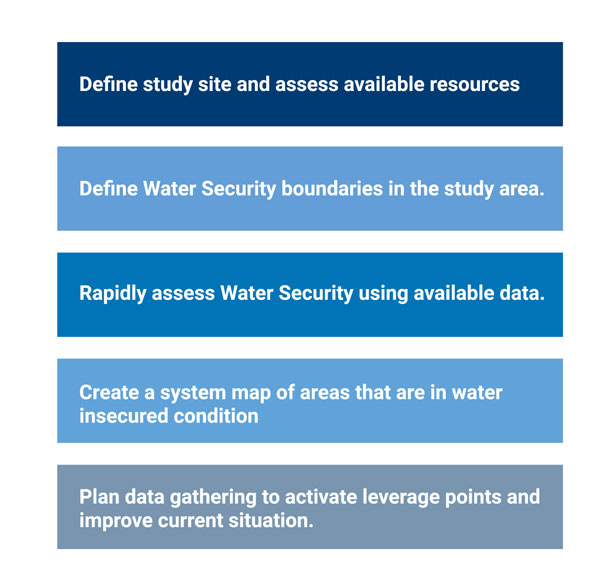
\includegraphics[width=0.4\linewidth]{images/WSCOAT_process}

\}

\textbackslash caption\{\emph{Proposed process to create a data gathering strategy} \}(\#fig:process diagram)
\textbackslash end\{figure\}

\hypertarget{intro}{%
\chapter{Identifying study site}\label{intro}}

\hypertarget{concepts}{%
\section{Concepts}\label{concepts}}

\hypertarget{tools}{%
\section{Tools}\label{tools}}

\textbf{River basin maps}
\href{https://hydrosheds.org}{Hydrosheds}

\hypertarget{an-example}{%
\section{An example}\label{an-example}}

The study was conducted on the Akaki River basin (Awash Wenz 2 in Hydrosheds REF). The catchment is located in central Ethiopia along the western mar- gin of the Main Ethiopian Rift and geographically located between 8°46´--9°14´N and 38°34´--39°04´E, covering an area of about 1500 km2. It experiences a temperate Afro-Alpine climate with daily average temperatures from 9.9 to 24.6 °C and annual mean rainfall is 1254 mm, as measured at Addis Ababa Observatory .Three main seasons can be observed: the major rainy one, locally known as Kiremt from June to September, contributing about 70\% of the total annual rainfall. A minor rainy season, locally known as Belg, from mid-February to mid-April. The remaining five months are dry season (Ethiopian Public health Institute, 2017).

\hypertarget{boundaries}{%
\chapter{WS boundaries}\label{boundaries}}

\hypertarget{concepts-1}{%
\section{Concepts}\label{concepts-1}}

The first step is to define the boundaries of Water Security (WS) in the studied area. To do so the approach proposed is to compare existing WS indexes.

\hypertarget{tools-1}{%
\section{Tools}\label{tools-1}}

\hypertarget{an-example-wq-for-akaki-river}{%
\section{An example: WQ for Akaki river}\label{an-example-wq-for-akaki-river}}

Add graph water quality

\hypertarget{identifying-sub-dimension-for-water-quality}{%
\subsection{Identifying sub-dimension for Water Quality}\label{identifying-sub-dimension-for-water-quality}}

Water quality was taken as an example on how to determine indicators for a given dimension. Five different indexes were compared (ADB, 2013; Babel and Shinde, 2013; Carden and Armitage, 2013; Hofste et al., 2019; Mason and Calow, 2012; UN-EP-DHI and UNEP, 2016) within the water quality dimension (Table 2). It can be observed how the used indicators converge to three distinct areas: assessment of river water quality (WQ01), groundwater quality (WQ02) and amount of treated discharge to the environment (WQ03). At a more detailed level, the indexes often use different parameters or methods.

\label{tab:unnamed-chunk-4}comparison of indicators used in different WS indexes to assess water quality.

Sub.dimension

Indicator

B2013

M2012

A3

TWAP

C2013

Discharges

Treated wastewater

NA

1

1

1

NA

Discharges

Wastewater management (RPMS -- KPI 6 / Green Drop)

NA

NA

NA

NA

1

Groundwater

Concentration of site-specific pollutants /Permissible limits of these pollutants

1

NA

NA

NA

NA

Groundwater

Groundwater quality (State report)

NA

NA

NA

NA

1

Surface water

Dissolved oxygen concentration/Permissible limit concentration

1

NA

NA

NA

NA

Surface water

Country-specific conditions (ADB, 2013)

1

NA

NA

NA

NA

Surface water

BOD 5-day values of river water samples. (Mehr, 2011)

1

NA

NA

NA

NA

Surface water

Change in percentage freshwater of samples meeting quality standards (from GEMS)

NA

1

NA

NA

NA

Surface water

Change in chlorophyll/ turbidity/ suspended solids; from MODIS satellite UN-Water EG-IMD (2009)

NA

1

NA

NA

NA

Surface water

Coastal eutrophication potential (CEP) s based on Billen and Garnier's (2007)

NA

NA

1

NA

NA

Surface water

Dissolved inorganic nitrogen (DIN) (sub-indicator 4a) b) , Dissolved inorganic phosphorous (DIP) (sub-indicator 4b)

NA

NA

NA

1

NA

Surface water

Water resource quality (River health, State report)

NA

NA

NA

NA

1

We have identified WQ sub-dimension as:

\hypertarget{identifying-indicators-for-each-sub-dimension}{%
\subsection{Identifying indicators for each sub-dimension}\label{identifying-indicators-for-each-sub-dimension}}

For each identified subdimension, a similar approach as previously adopted was carried. \textbf{WQ01: parameters used for river water health assessment.} To better understand the range of possible parameters, a comparison was carried across previously published studies (Banda and Kumarasamy, 2020; Keraga et al., 2017; Melaku et al., 2007; Troyer et al., 2016; Worako, 2015; Yilma et al., 2018; Zotou et al., 2018). Additionally, five studies were found to use macroinvertebrate indexes to assess water quality (Akalu, S., Mengistou, S., and Leta, 2011; Aschalew and Moog, 2015; Beyene et al., 2009; Desalegne, 2018; Kebede et al., 2020). Table 3 shows the result of the analysis. The number of parameters used ranged from a minimum of 7 to maximum of 36. Overall the considered studies used a total of 59 parameters and 3 macroinvertebrates indexes. A set of parameters has been used in at least half of the considered studies (frequency \textgreater7): pH,DO,EC,Temp,NO3, BOD5, NH3, PO4.

\label{tab:unnamed-chunk-5}comparison of indicators used in different WS indexes to assess water quality.

ï..Indicator

F

C1

C2

C3

C4

C5

C6

C7

C8

C9

C10

C11

C12

C13

pH

10

1

1

1

1

1

1

1

1

1

1

DO

9

1

1

1

1

1

1

1

1

1

EC

9

1

1

1

1

1

1

1

1

1

Temp

9

1

1

1

1

1

1

1

1

1

NO3

8

1

1

1

1

1

1

1

1

BOD5

7

1

1

1

1

1

1

1

NH3

7

1

1

1

1

1

1

1

PO4

7

1

1

1

1

1

1

1

TSS

6

1

1

1

1

1

1

Cl-

5

1

1

1

1

1

TDS

5

1

1

1

1

1

Turb

5

1

1

1

1

1

Ca

4

1

1

1

1

COD

4

1

1

1

1

Alk

3

1

1

1

F

3

1

1

1

Macroinv. ETHbios

3

1

1

1

Mg

3

1

1

1

Mn

3

1

1

1

NO2

3

1

1

1

SO4

3

1

1

1

TOC

3

1

1

1

TH index

3

1

1

1

Chl-a

2

1

1

Cr

2

1

1

Cu

2

1

1

E.coli

2

1

1

Fe

2

1

1

K

2

1

1

Macroinvert SASS5

2

1

1

Na

2

1

1

NH4-N

2

1

1

Ni

2

1

1

Pb

2

1

1

SAR

2

1

1

TN

2

1

1

TP

2

1

1

Zn

2

1

1

CaCO3

1

1

Cd

1

1

Cl2

1

1

CO3 2-

1

1

DO\%

1

1

Enterococci

1

1

FC

1

1

HCO3

1

1

KR

1

1

Macroinver. TARISS

1

1

Macroinv. (other)

1

1

Macroinv. and diatoms

1

1

MAR

1

1

QHEI

1

1

RSC

1

1

S2-

1

1

Salinity

1

1

SiO2

1

1

SRP

1

1

SSP

1

1

TAN tot amm nitrogen

1

1

\hfill\break

\textbf{WQ02: parameters used for groundwater assessment} -- The same process was followed for groundwater. Parameters used in five published studies in Ethiopia were compared (Table 4). Much more agreement between studies was found in the choice of parameters. The number of parameters used in each study varied from 13 to 16. A core dataset of twelve parameters was identified since it was used over 80\% of the times.

\label{tab:unnamed-chunk-6}comparison of indicators used in different WS indexes to assess water quality.

Indicator

Frequency

Ka18

Di20

Fe20

To20

Be19

Ca

5

1

1

1

1

1

Cl-

5

1

1

1

1

1

EC

5

1

1

1

1

1

F

5

1

1

1

1

1

HCO3

5

1

1

1

1

1

K

5

1

1

1

1

1

Mg

5

1

1

1

1

1

Na

5

1

1

1

1

1

pH

5

1

1

1

1

1

SO4

5

1

1

1

1

1

NO3

4

1

1

1

1

TDS

4

1

1

1

1

CO3 2-

2

1

1

Fe

2

1

1

TH index

2

1

1

B

2

1

1

\hfill\break

\textbf{WQ03 Treated wastewater} -- The last indicator is usually estimated using national or municipality level available data. In some cases, a Shit Flow Analysis (sfd.susana.org) may exist. At national level, FAO estimated 0.3\% of treated municipal wastewater (FAO, 2016). It the case of Addis Ababa, an estimate of 7\% wastewater treatment was published by the Ministry of Water and Electricity (MoWIE, 2017).

\includegraphics{WSCOAT_files/figure-latex/Water Security-1.pdf}

\hypertarget{water-security-rapid-assessment}{%
\chapter{Water Security rapid assessment}\label{water-security-rapid-assessment}}

\hypertarget{concepts-2}{%
\section{Concepts}\label{concepts-2}}

Using available data

\hypertarget{tools-2}{%
\section{Tools}\label{tools-2}}

\hypertarget{an-example-1}{%
\section{An example}\label{an-example-1}}

The rapid assessment on available data gave this result:

\label{tab:unnamed-chunk-7}comparison of indicators used in different WS indexes to assess water quality.

ï..Empty

Dimension

Sub.dimension

Status

NA

Climate

Variability

1

NA

Climate

Drought

3

NA

Water Quality

Wastewater treatment

4

NA

Water Quality

River water health

4

NA

Water Quality

Groundwater quality

2

NA

Efficiency / Economic Value

Agriculture

3

NA

Efficiency / Economic Value

Industry

3

NA

Sanitation

health

3

NA

Sanitation

services

4

NA

Socio-economic

growth

3

NA

Socio-economic

vulnerability

4

NA

Governance

Legislation

2

NA

Governance

Implementation

4

NA

Damages

Economic loss

2

NA

Damages

Casualties

2

NA

Finance

Available budget

3

NA

Supply-demand

withdrawal

3

NA

Supply-demand

mitigation capacity

2

NA

Supply-demand

supply infrastructure

2

\hypertarget{water-security-system-map}{%
\chapter{Water Security system map}\label{water-security-system-map}}

Some \emph{significant} applications are demonstrated in this chapter.

\hypertarget{concepts-3}{%
\section{Concepts}\label{concepts-3}}

\hypertarget{tools-3}{%
\section{Tools}\label{tools-3}}

\hypertarget{an-example-2}{%
\section{An example}\label{an-example-2}}

The findings of the rapid assessment on water quality were visualized using the diagram developed during the Hub assembly in Ethiopia (Figure 4). The natural environment (N) is under stress due to discharges from anthropogenic activities and growing urbanization (axis GU-P-I-N). Low environmental awareness (AW) and a weak governance in implementing existing regulation (G) does not create a sufficient barrier to reduce pressure on the environment. This condition has implie The poor quality or river water and ecosystem has negative impact on population health(N-P) and economic resources (N-R).Low environmental awareness (AW) and a loose implementation of existing regulation does not reduce

\hypertarget{data-gathering-strategy}{%
\chapter{Data gathering strategy}\label{data-gathering-strategy}}

\hypertarget{concepts-4}{%
\section{Concepts}\label{concepts-4}}

The data gathering process was divided into three sets of decision: where (Location), when (Frequency) and what to sample (Parameter). Additionally available resources ( budget, time, capacity, access) should be considered. In the example,\\
In the following paragraphs, an incremental approach is suggested with different approaches based on available data.

Another important

\hypertarget{location}{%
\subsection{Location}\label{location}}

The choice of sampling location can be determined based on the available information. The incremental approach proposed develops on three levels (L1,L2,L3)

\textbf{L1: Topological approach} -- The choice of sampling location is one of the first decision to be taken. In case of no prior information the topological approach developed by \citet{Sharp1971}. This method allows to optimize network coverage and sampling points with only the network topology. Each section of the river is numbered based on the number of tributaries (or sources) that is receiving. Applying this procedure to a network creates a magnitude value for each segment. Centroid position can defined as the segment nearest to \(M_o/2\), where \(M_o\) is the magnitude at the outlet. This step can be repeated several to meet a desired number of sampling locations (figure \ref{fig:sharp01}).

It is recommended to sample after full water mixture, a distance from tributaries connection of L=25 x width can be taken as general reference \citep{Alilou2019}.

\textbackslash begin\{figure\}

\{\centering 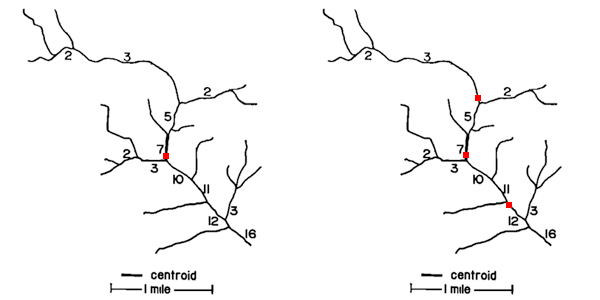
\includegraphics[width=0.6\linewidth]{images/sharp01}

\}

\textbackslash caption\{\emph{Figure 1: assigning a magnitude value for each segment based on its tributaries. The centroid is located (left image)at the nearest segment of \(M_o/2\). In this case segment with magnitude 7, since 16/2=8. The network would be divided into two segments of magnitude 7 and 9 (given by 16-7). With the same procedure the following sampling points would be determined near the half magnitude of each segment (on the right)} . Source: \citet{Sharp1971}\}\label{fig:sharp01}
\textbackslash end\{figure\}\\

\textbf{L2: Weighted topological approach based on land cover} -- After the first draft of ideal location points, new knowledge can be incorporated in form of expert opinion, published literature, national data. The topological approach was improved by associating weight to each river segment \citep[ ]{Sanders1983, Rajagopal1983}.

\hfill\break

\textbf{L3 incorporating published literature} -- Data from published studies \citep{Akalu2011, Melaku2007, Kassegne2019, Weldegebriel2012}. (Figure 8.4) was used to update the map (Figure 8.5) by ranking the river segments based on risk likelihood. Likelihood was calculated as assumed water quality x presence of farming activities. Note that farming was only assessed as presence/absence and size of farmed land was not considered.

\hfill\break

\textbf{L4 using geo-statistical tools} -- Moving towards more sophisticated methods, kriging, genetic algorithm, conditional entropy could be included (Jiang et al., 2020; Karamouz et al., 2009) as well as Bayesian approaches (Scientific Advisory Board-Ecological Processes Standing Committee (EPSC), 2014). This would require initial data from existing stations and a higher capacity for calculations.

\hypertarget{frequency}{%
\subsection{Frequency}\label{frequency}}

Frequency of sampling is likely to be determined by project timeline and budget. Despite this limitation, some considerations can be made.

\textbf{F1 minimum requirement} -- A bare minimum could consist in one sample per location per climatic season.

\textbf{F2 minimum international standard} -- The program GEMS/WATER recommends for streams an optimal of 24 samples per year (with a minimum of 4) and a minimum of 12 and maximum of 24 for large drainage areas of rivers (100,000 km2).

\textbf{F3 frequency for hypothesis testing} -- Once previously published data is incorporated, sampling number and frequency can be adjusted to detect a specific margin or trend. For a given confidence (\(Z_α/2\)), previously calculate mean (µ) and variance (σ) and confidence interval width (\(µ-x\)) \citep{Sanders1983}{[}eq. 5.7{]} Sanders (1983 eq. 5.7; \citet{Sanders1978} Sanders and Adrian, 1978) proposes the following:

\[n≥\left(\frac{Z_{α/2}\times σ}{μ-x}\right)^2\]

For time series a quantification of samples that assumes concentrations to be random, independent and identically distributed would be calculated as (Strobl and Robillard, 2008):

\[N=[(t_{α/2} S / R)]\times2\]

Where N is the number of equally (temporally) spaced samples collected per year; tα/2 is a constant which is a function of the level of significance, and the number of samples; S is the standard deviation of the water quality concentrations; and R is the specified half-width of the confidence interval of the annual mean.
More sophisticated statistical tools can be used including harmonic, Bayesian analysis, entropy, semivariogram (Khalil and Ouarda, 2009).

\hypertarget{parameters}{%
\subsection{Parameters}\label{parameters}}

\hypertarget{tools-4}{%
\section{Tools}\label{tools-4}}

\hypertarget{an-example-3}{%
\section{An example}\label{an-example-3}}

\hypertarget{location-1}{%
\subsection{Location}\label{location-1}}

\hypertarget{frequency-1}{%
\subsection{Frequency}\label{frequency-1}}

\hypertarget{parameters-1}{%
\subsection{Parameters}\label{parameters-1}}

\begin{Shaded}
\begin{Highlighting}[]
\NormalTok{akaki\_WQ }\OtherTok{\textless{}{-}} \FunctionTok{read.csv}\NormalTok{(}\StringTok{"./data/Akaki\_WQ.csv"}\NormalTok{)}
\end{Highlighting}
\end{Shaded}

\citet{Kassegne2019}

  \bibliography{datagathering.bib}

\end{document}
